
%(BEGIN_QUESTION)
% Copyright 2008, Tony R. Kuphaldt, released under the Creative Commons Attribution License (v 1.0)
% This means you may do almost anything with this work of mine, so long as you give me proper credit

Small relays often come packaged in clear, rectangular, plastic cases.  These so-called ``ice cube'' relays have either eight or eleven pins protruding from the bottom, allowing them to be plugged into a special socket for connection with wires in a circuit.  Note the labels near terminals on the relay socket, showing the locations of the coil terminals and contact terminals:

$$\includegraphics[width=15.5cm]{i03210x01.eps}$$

Draw the necessary connecting wires between terminals in this circuit, so that actuating the normally-open pushbutton switch sends power from the battery to the coil to energize the relay, with one of the relay's normally-open contacts turning the lamp on.  The pushbutton switch should not carry any lamp current, just enough current to energize the relay coil:

\vskip 20pt

$$\includegraphics[width=15.5cm]{i03210x02.eps}$$

\vfil 

\underbar{file i03210}
\eject
%(END_QUESTION)





%(BEGIN_ANSWER)

This is a graded question -- no answers or hints given!
 
%(END_ANSWER)





%(BEGIN_NOTES)

An excellent problem-solving strategy to apply in cases such as this is to first sketch a proper {\it schematic} diagram before attempting to complete a pictorial diagram.  Schematics are easier to follow than pictorial diagrams because you have the freedom to position components as you see fit, rather than be forced to draw the wires with the components in the given positions.  Here I show what a schematic diagram for this circuit might look like (note that there are multiple correct answers here, and that this particular schematic is not the only proper solution):

$$\includegraphics[width=15.5cm]{i03210x04.eps}$$

\vskip 10pt

Based on this clear and easy-to-follow schematic diagram, I can now sketch a working solution in pictorial form:

$$\includegraphics[width=15.5cm]{i03210x03.eps}$$

%INDEX% Pictorial circuit review (relay circuit)

%(END_NOTES)


